\documentclass{ecnreport}

\stud{Option Robotique, Control \& Robotics master}
\topic{Advanced Robot Programming}

\begin{document}

\inserttitle{Advanced Robot Programming  Labs \newline C++ Programming}

\insertsubtitle{Lab 2: Mobile robot with sensors}


\section{Content of this lab}

The goal of this lab is to read, use and build C++ classes in order to develop an elementary simulator for a ground robot.

\subsection{The simulator}

The simulator is defined by several headers and source files, as defined in \Fig{fig:dirtree}.
\begin{figure}[h]
\begin{minipage}{.25\linewidth} ~ \end{minipage}
\begin{minipage}{.5\linewidth}
 \dirtree{%
.1 lab2.
.2 CMakeLists.txt.
.2 include.
.3 envir.h.
.3 geom.h.
.3 robot.h.
.3 sensor.h.
.2 src.
.3 envir.cpp.
.3 main.cpp.
.3 robot.cpp.
} 
\end{minipage}
%\begin{minipage}{.2\linewidth} ~ \end{minipage}
\caption{\label{fig:dirtree} Files used by the simulator}
\end{figure}

The main file is \texttt{main.cpp} and is compiled to an executable.\\
The files \texttt{robot.h} and \texttt{robot.cpp} define a \texttt{Robot} class and will be modified in the first lab to implement new methods that allow using the simulator.

The files \texttt{envir.h} and \texttt{envir.cpp} defines the environment in which the robot is moving. These files are not to be modified.

The file \texttt{sensor.h} defines a virtual class \texttt{Sensor} that will be used to create two sensor types: range and bearing sensors.

\subsection{If you do the lab on your own computer}

You of course have to install QtCreator and CMake:\\
\texttt{sudo apt-get install cmake qtcreator} \\

You will also have to install these Ubuntu packages that are used for the plotting of the robot trajectory:\\
\texttt{sudo apt-get install python-matplotlib}

\subsection{Expected work}

During the lab the files will be modified and others will be created.
At the end of the lab, please send by email a zip file allowing to compile and test the program.

You may answer the questions by inserting comments in the code at the corresponding lines.

\subsection{Geometry structures}

In the \texttt{geom.h} file are defined two simple geometry structures:
\begin{itemize}
 \item One for a 2D pose: \texttt{Pose} with attributes \texttt{x, y, theta}
 \item One for a 2D motion: \texttt{Twist} with attributes \texttt{vx, vy, w} 
\end{itemize}Those structures have classical constructors, and also methods to express change of frames:
\begin{itemize}
 \item \texttt{Pose Pose::transformDirect(Pose \_transform)} \\returns the pose  expressed in the given transform
 \item \texttt{Pose Pose::transformInverse(Pose \_transform)}\\ returns the pose expressed in the given transform inverse
 \item \texttt{Twist Twist::transformDirect(Pose \_transform)} \\returns the twist expressed in the given transform
 \item \texttt{Twist Twist::transformInverse(Pose \_transform)}\\ returns the twist expressed in the given transform inverse
 \end{itemize}


\newpage

\begin{figure}\centering
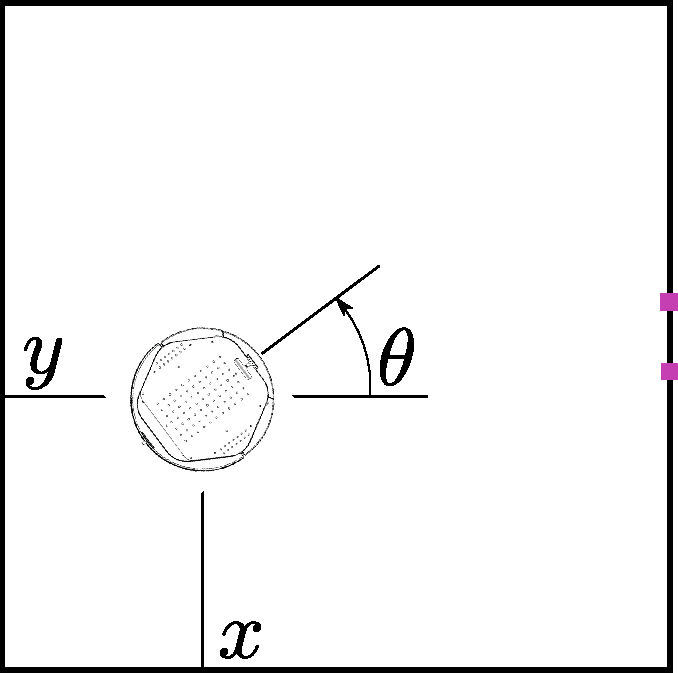
\includegraphics[width=.3\linewidth]{environment}
\caption{\label{fig:envir} Robot in its environment}
\end{figure}


\section{Building the \texttt{Robot} class}

The default behavior is the robot following a moving target in the environment. The environment consists of 4 walls defining a 20$\times$20 m square. The target is leaving the square at some point, 
and for now the robot is also leaving the square as nothing tells it that there are some walls there.

\subsection{Defined methods}

Some methods of the class are already defined:
\begin{itemize}
 \item \texttt{Robot(std::string \_name, double \_x, double \_y, double \_theta)}\\
 constructor, initialize the robot with a given name at a given $(x,y,\theta)$ position
 \item \texttt{Pose pose()} \\ returns the current pose of the robot
 \item \texttt{void moveXYT(double \_vx, double \_vy, double \_omega)}\\
 sends a $(v_x, v_y, \omega)$ velocity to the robot and updates its position
 \item \texttt{void goTo(const Pose \&\_p)}\\
 tries to have the robot reach the given Pose
\end{itemize}


\subsection{Incomplete methods}


\begin{itemize}
\medskip\item[\textbf{\underline{Q1}}]  Compile and execute the program. According to the \texttt{main.cpp} file, the robot is trying to go to the position of the target. In which files is the target motion defined?

\medskip\item[\textbf{\underline{Q2}}] Explain the signature of   \texttt{Robot::Robot}, especially the way to pass arguments.

\medskip\item[\textbf{\underline{Q3}}] In practice it is often impossible to control a ground robot by sending $(x,y,\theta)$ velocities. A classical way to control such a robot is to send a setpoint with a linear velocity $v$ and an angular velocity $\omega$, expressed in the robot frame as shown in \Fig{fig:dd}.

\begin{figure}[h!]\centering
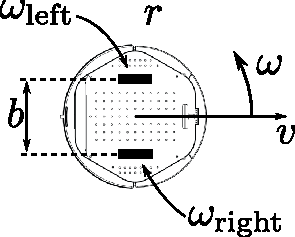
\includegraphics[width=.3\linewidth]{wheels}
\caption{\label{fig:dd} Differential drive model}
\end{figure}

The corresponding model is quite simple:
\begin{equation*}
\left\{\begin{array}{ll}
\dot x &= v\cos \theta \\
\dot y &= v\sin \theta \\
\dot \theta &= \omega
\end{array}\right.
\end{equation*}

Implement such a function in \texttt{Robot::moveVW}. This method should compute the $(x,y,\theta)$ velocities from $(v,\omega)$ and then call the \texttt{Robot::moveXYT} method. 

\medskip\item[\textbf{\underline{Q4}}] Now that a realistic way to control the robot is possible, should the \texttt{Robot::moveXYT} method stay available for external use? What can we do in the \texttt{robot.h} file to make it impossible to use it from outside the \texttt{Robot} class?

\medskip\item[\textbf{\underline{Q5}}] The \texttt{moveWithSensor} method was using the XYT motion, which is not realistic. 
Modify it so that it calls the \texttt{moveVW} method. A simple way to change a desired $(\dot x, \dot y, \dot \theta)$ motion
to a $(v, \omega)$ motion is:
\begin{equation*}\left\{\begin{array}{ll}
 v& = \dot x\\
 \omega &= \alpha\dot y + \dot \theta\end{array}\right.
\end{equation*}We will use $\alpha = 20$ here.

\medskip\item[\textbf{\underline{Q5}}] When a robot is equipped with two actuated wheels, a simple model is the differential drive model, as shown in \Fig{fig:dd}. Assuming the two wheels have a radius $r$ and are separated with a distance $b$, then the kinematic model yields:
\begin{equation*}\label{eq:dk}
\left\{\begin{array}{ll}
v &= \displaystyle r \frac{\omega_l + \omega_r}{2} \\
\omega &= \displaystyle r \frac{\omega_l - \omega_r}{2b}
\end{array}\right.
\end{equation*}
We will need to define new attributes in the \texttt{Robot} class in order to initialize the radius and base distance.
Create also a new method in the \texttt{Robot} class, called \texttt{initWheel}, that does so. In the \texttt{main.cpp}, use the following values:
\begin{equation*}
\left\{\begin{array}{ll}
r &= 0.07 ~m \\
b &= 0.3 ~m
\end{array}\right.
\end{equation*}

\medskip\item[\textbf{\underline{Q6}}] Now that the robot has some wheel radius and inter-distance, implement the \texttt{Robot::rotateWheels} method, so that it can be possible to control the robot by sending wheel velocities. 
The method should call \texttt{Robot::moveXYT} after having computed the $(x,y,\theta)$ velocities from $(\omega_l, \omega_r)$.

\medskip\item[\textbf{\underline{Q7}}] By using a \texttt{bool wheels\_init\_} attribute, make sure that it is impossible to do anything in \texttt{Robot::rotateWheels} if the radius and base have not been initialized.

\subsection{Velocity limits}

With the current simulation, we can control the robot:
\begin{itemize}
\item by sending linear and angular velocity setpoint with \texttt{Robot::moveVW}
\item or by sending wheel velocities with \texttt{Robot::motateWheels}
\end{itemize}

These two methods call \texttt{Robot::moveXYT}\footnote{which should not be calable anymore from outside the \texttt{Robot} class} and the robot can reach any velocity. In practice, the wheels have a limited velocity at $\pm$10 rad/s.

\medskip\item[\textbf{\underline{Q1}}] Modify the \texttt{Robot::initWheels} method in order to pass a new argument that defines the wheel angular velocity limit.
You may need to define a new attribute of the \texttt{Robot} class to store this limit.

\medskip\item[\textbf{\underline{Q2}}] Modify the \texttt{Robot::rotateWheels} method in order to ensure that the applied velocities $(\omega_l, \omega_r)$ are within the bounds.
The method should also print a message if the velocity setpoint is too high.
Note that if you just saturate the velocities, the robot motion will be different.
A scaling is a better strategy, in this case we keep the same ratio between $\omega_l$ and $\omega_r$ according to the following algorithm:

\def\wl{\omega_l}
\def\wr{\omega_r}
\def\wm{\omega_{\text{max}}}

\begin{algorithm}[!h]
\SetKwComment{Comment}{(}{)}
% \SetAlgoLined
\KwData {desired wheel velocities $\wl$, $\wr$, velocity limit $\wm$}
\KwResult {actual velocities $\wl$, $\wr$}
$a\gets$ max($|\wl|/\wm$,$|\wr|/\wm$)\;
\If{$a <$ 1}{$a\gets$1\;}
\Return $\wl/a$, $\wr/a$\;
\caption{Scale wheel velocities with maximum value}
\label{algo:grad}
\end{algorithm}


\medskip\item[\textbf{\underline{Q3}}] Although the robot actually moves by having its wheels rotate, 
it is more natural to send linear and angular velocity setpoints. Modify the 
\texttt{Robot::moveVW} method so that a $(v,\omega)$ setpoint is changed to a $(\omega_l,\omega_r)$ setpoint that will then be called through \texttt{Robot::rotateWheels}.
 The inverse of model \eqref{eq:dk} yields:
\begin{equation}
\left\{\begin{array}{ll}
\omega_l &= \displaystyle \frac{v + b\omega}{r} \\
\omega_r &= \displaystyle \frac{v - b\omega}{r}
\end{array}\right.
\end{equation} 
The corresponding behavior should be that the robot cannot follow perfectly the target anymore, because it is not fast enough.
\end{itemize}

% \begin{figure}[h!]
% 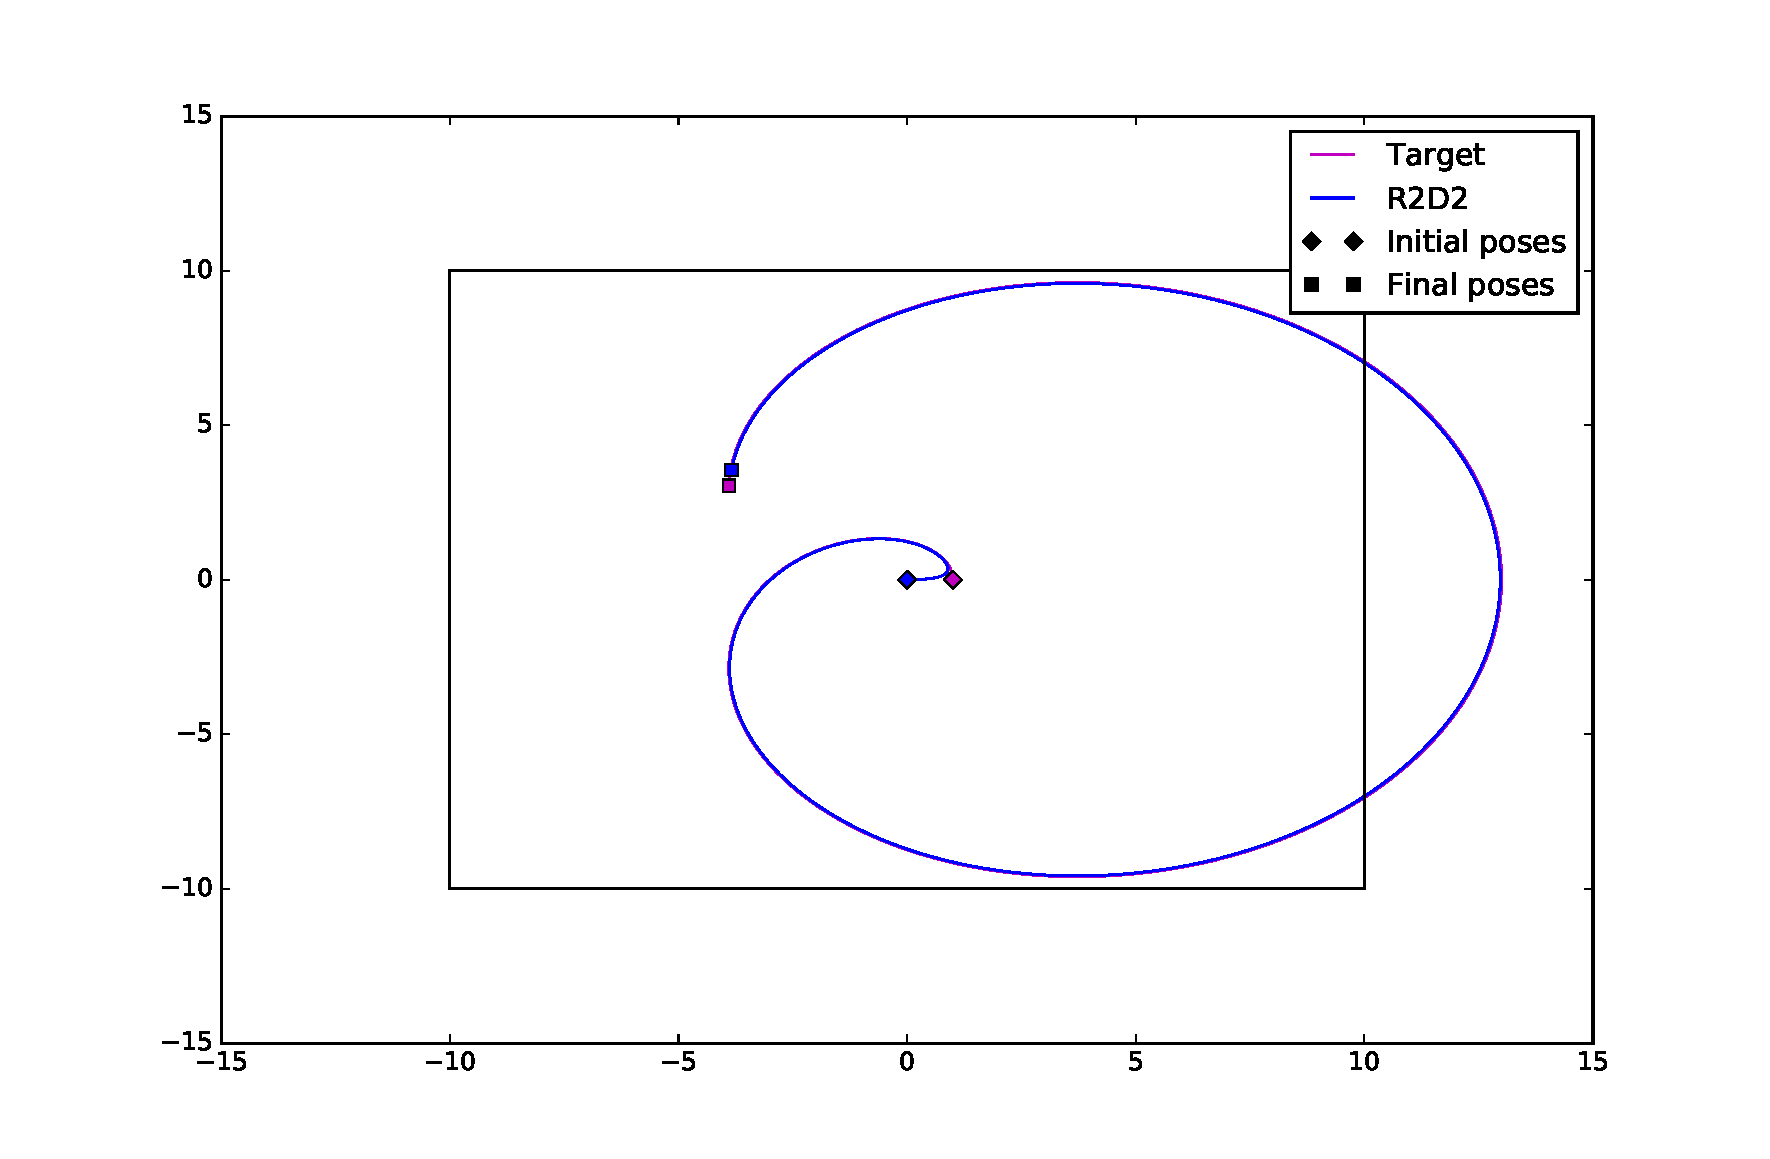
\includegraphics[width=.4\linewidth]{xyt} \quad 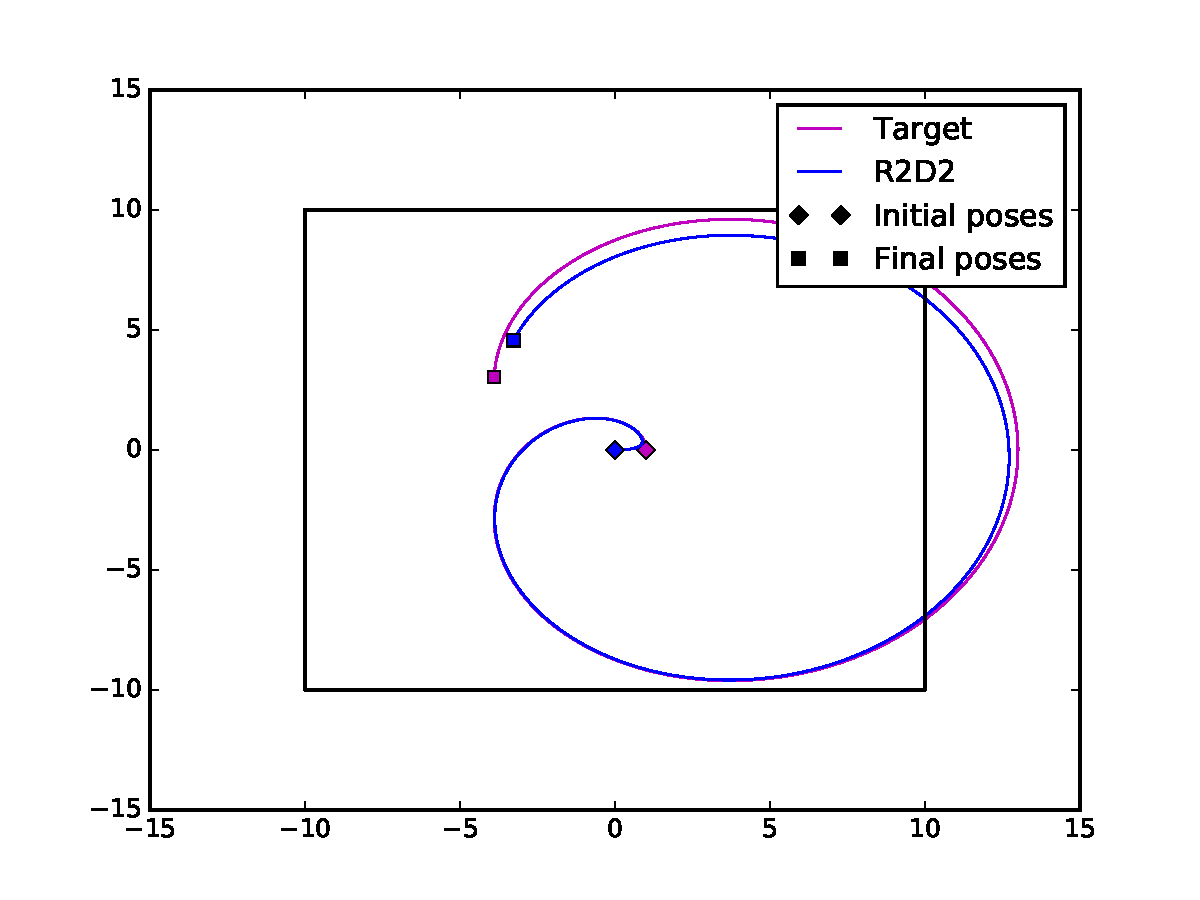
\includegraphics[width=.4\linewidth]{vw} 
%  
% \end{figure}
\newpage

\section{Sensors}

In this section we will try to avoid the walls by using some range sensors.

The \texttt{sensor.h} files defines a \texttt{Sensor} class that has the following methods:
\begin{itemize}
\item \texttt{Sensor(Robot \&\_robot, double \_x, double \_y, double \_theta)}\\initializes a sensor at a given position on the given robot
\item \texttt{virtual void update(const Pose \&\_p)}\\ updates the measurement from the sensor current position
\item \texttt{virtual void correctTwist(Twist \&\_v)}\\ checks if the given Twist is fine with the current sensor measurement
\item \texttt{void updateFromRobotPose(const Pose \&\_p)}\\ computes the sensor absolute position from the given robot pose, then calls \texttt{update}
\item \texttt{void correctRobotTwist(Twist \&\_v)}\\ computes the twist in the sensor space, then calls \texttt{correctTwist}
\end{itemize}
Some of the methods are pure virtual functions, which makes the \texttt{Sensor} class an abstract class.
It is thus impossible to declare a variable to be of \texttt{Sensor} type, as this class is only designed to build daughter-classes depending on the sensor type.

The \texttt{Robot} class already has a attribute called \texttt{sensors\_} which is a vector of \texttt{Sensor*}.

For example to update all sensors with the current robot pose, we can write the following:
\begin{center}\cppstyle
\begin{lstlisting}
    for(auto & sensor: sensors_)
	sensor->updateFromRobotPose(pose_);
\end{lstlisting}
\end{center}The arrow is because we use a pointer and not an actual value. The corresponding methods have thus to be 
called with an arrow instead of a dot.





\subsection{Range sensor}


\begin{itemize}
\medskip\item[\textbf{\underline{Q1}}] Create a \texttt{sensor\_range.h} file that defines a \texttt{RangeSensor} class that is derived from \texttt{Sensor}. The \texttt{update} and \texttt{correctTwist} methods have to be defined so that the code compiles. For now, just make the methods print something to the screen.
As the \texttt{Sensor} class does not have a default constructor, the \texttt{RangeSensor} class must have its constructor call directly the one from  \texttt{Sensor}:
\begin{center}\cppstyle
\begin{lstlisting}
class RangeSensor : public Sensor
{
public:
    RangeSensor(Robot &_robot, double _x, double _y, double _theta) :
	Sensor(_robot, _x,  _y,  _theta) // call the Sensor constructor
        {}	// the RangeSensor constructor does nothing more
};    
\end{lstlisting}
\end{center}

\medskip\item[\textbf{\underline{Q2}}] Include this file in \texttt{main.cpp} and declare a \texttt{RangeSensor} variable.  We will use a front range sensor placed at $(0.1, 0,0)$ in the robot frame.

\medskip\item[\textbf{\underline{Q3}}] In the \texttt{Robot::moveWithSensor} method we currently do not take into account the sensor measurement. 
Before calling \texttt{moveVW} we should loop through all the sensors of the robot and call their \texttt{updateFromRobotPose} method.

\medskip\item[\textbf{\underline{Q4}}] In this question we will build the \texttt{update} function of the range sensor.
This sensor should compute the distance to the nearest wall in the direction of the x-axis.\\

In the \texttt{envir\_} attribute of the sensor class, the walls are defined by a list of points available in \texttt{envir\_->walls}. \Fig{fig:dist} shows a configuration where the sensor is at $(x,y,\theta)$ and is facing a wall defined by $(x_1,y_1)$ and $(x_2,y_2)$.
\begin{figure}[h]\centering
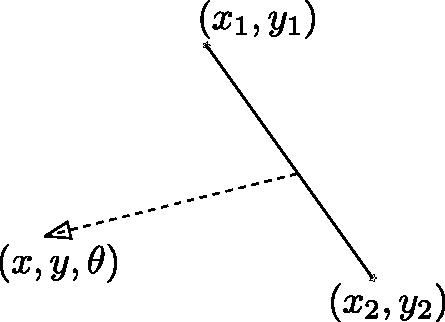
\includegraphics[width=.3\linewidth]{sensor}
\caption{Distance to a segment defined by two points.}
\label{fig:dist}
\end{figure}
In this case, the distance to the wall is:
\begin{equation}
d = \frac{x_{1} y_{2} - x_{1} y - x_{2} y_{1} + x_{2} y + x y_{1} - x y_{2}}{x_{1} \sin\theta - x_{2} \sin\theta - y_{1} \cos\theta + y_{2} \cos\theta}
\end{equation}
The computed distance is positive if the wall is in front of the sensor, and negative if it is behind (in this case this wall is actually not measured). Also, the denominator may be null if the wall is parallel to the sensor orientation.

A simple code to loop trough all the walls is:
\begin{center}\cppstyle
\begin{lstlisting}
Pose p1, p2;
for(int i=0;i<envir_->walls.size();++i)
{
    p1 = envir_->walls[i];
    p2 = envir_->walls[(i+1)%envir_->walls.size()];

    // do whatever you want to do with points p1 and p2
}
\end{lstlisting}
\end{center}

Define the \texttt{update} function so that it updates the attribute \texttt{s\_} of the sensor with the distance to the nearest wall. Make it also print the distance to see if it is fine.

\medskip\item[\textbf{\underline{Q5}}] We now want the sensor to be able to modify the robot twist to prevent any collisions, which is the goal of the \texttt{correctTwist} method.
We assume the \texttt{Twist} that is passed to this method is already expressed in the sensor frame. Hence we are only interested in the \texttt{vx} attribute and do not want it to be too large (fast motion in the sensor axis) if we are near to a wall.\\
A simple way to do so is to define a minimum security range and to impose an upper bound to the velocity:

\medskip\item[\textbf{\underline{Q6}}] Modify the \texttt{Robot::moveWithSensor} method so that we also check the current robot twist by calling the \texttt{correctRobotTwist} method for all sensors. The robot should then stay inside the walls. We will use the following parameters:
\begin{equation*}
\left\{\begin{array}{ll}
g &= .1 \\
s_m &= 0.1~ m
\end{array}\right.
\end{equation*}

\begin{algorithm}[!h]
\SetKwComment{Comment}{(}{)}
% \SetAlgoLined
\KwData {Current twist $T$, current range $s$, gain $g$, minimum range $s_m$}
\KwResult {Modified twist $T$}
\If{$T.vx > g*(s-s_m)$}{$T.vx \gets g*(s-s_m)$\;}
\Return $T$
\caption{Modify the given twist to avoid collisions}
\label{algo:range}
\end{algorithm}
\medskip\item[\textbf{\underline{Q7}}] Add some other range sensors to the robot to check if everything is going fine.
\end{itemize}



\newpage

\subsection{Bearing sensor}

In this section we will create a new kind of sensor, that returns the bearing angle to the other robot in the simulation.
Define first a new robot with smaller wheels (0.05 m). \\
In the main loop, we just want this robot to go forward at 0.4 m/s: \\\texttt{robot2.moveWithSensor(Twist(0.4,0,0));}\\
Of course it will go out of the wall for now.

\begin{itemize}
\medskip\item[\textbf{\underline{Q1}}] Create a \texttt{sensor\_bearing.h} file that defines a \texttt{SensorBearing} class that is derived from \texttt{Sensor}. The \texttt{update} and \texttt{correctTwist} methods have to be defined so that the code compiles. For now, just make the methods print something to the screen.

\medskip\item[\textbf{\underline{Q2}}] Include this file in \texttt{main.cpp} and declare a \texttt{SensorBearing} variable.  We will use a front bearing sensor placed at $(0.1, 0,0)$ in the second robot frame.

\medskip\item[\textbf{\underline{Q3}}] Here we build the \texttt{update} method. The sensor measurement should be the angle under which the sensor is detecting another robot. 
We have to loop through all the robots of the environment, which can be done with this loop:
\begin{center}\cppstyle
\begin{lstlisting}
// look for first other robot
    for(auto other: envir_->robots_)
	if(other != robot_)
	{
	    // compute angle between sensor and detected robot
	    
	    break;
	}
    // set angle back to [-pi,pi]
\end{lstlisting}
\end{center}
The angle between the sensor and the robot can be computed with:
\begin{equation*}
 \alpha = \text{arctan2}(y_r - y_s, x_r-x_s) - \theta_s
\end{equation*}where $(x_s,y_s,\theta_s)$ is the sensor pose and $(x_r,y_r)$ is the robot position.

\medskip\item[\textbf{\underline{Q4}}] We now build the \texttt{correctTwist} method. The bearing sensor should try to align with its target. To do so, we just want to change the rotation velocity:
\begin{algorithm}[!h]
\SetKwComment{Comment}{(}{)}
% \SetAlgoLined
\KwData {Current twist $T$, current bearing $s$, gain $g$}
\KwResult {Modified twist $T$}
$T.w \gets T.w - g\times s$\;
\Return $T$
\caption{Modify the given twist to avoid collisions}
\label{algo:bearing}
\end{algorithm}

We use this method with the following parameters: $g = 0.5$.


\medskip\item[\textbf{\underline{Q5}}] Check that the second robot now follows the first robot, just by using its bearing sensor. 

\end{itemize}

\end{document}
